% gr-Kneser.tex -- the Petersen graph is the Kneser graph K(5,2)
% vertices : the 2-subsets of {1,...,5} ; two subsets are adjacent
% when they are disjoint. Engine : pdfLaTeX or LuaLaTeX
\documentclass[border=3mm, convert=false]{standalone}
\usepackage{tkz-berge}
\begin{document}
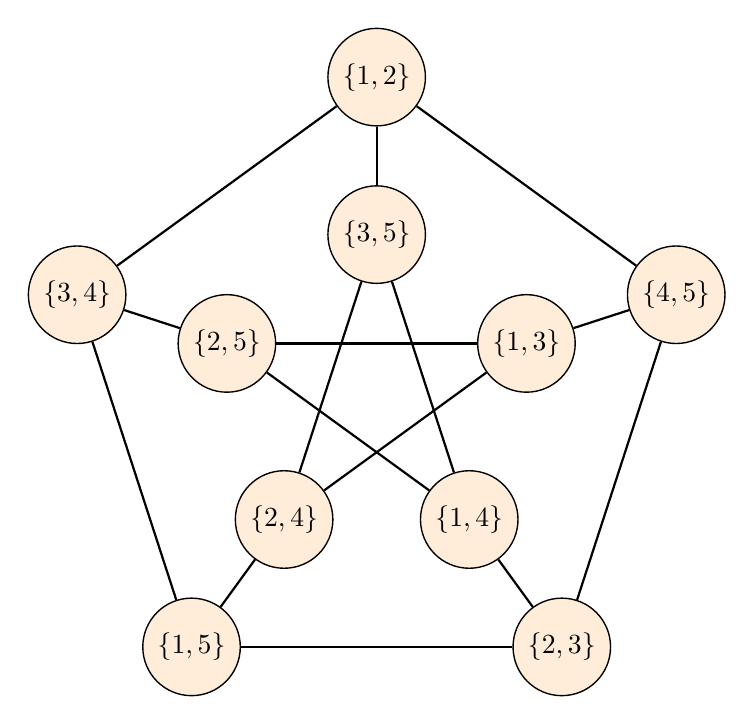
\begin{tikzpicture}
  \GraphInit[vstyle=Normal]
  \tikzset{VertexStyle/.append style = {minimum size = 26pt,
                                         fill = orange!15}}
  \SetVertexMath
  % outer pentagon and inner pentagram
  \foreach \a/\b/\k in {1/2/0,3/4/1,1/5/2,2/3/3,4/5/4}
    {\Vertex[a=90+72*\k,d=4,L={\{\a,\b\}}]{\a\b}}
  \foreach \a/\b/\k in {3/5/0,2/5/1,2/4/2,1/4/3,1/3/4}
    {\Vertex[a=90+72*\k,d=2,L={\{\a,\b\}}]{\a\b}}
  % an edge between two disjoint subsets
  \foreach \a/\b in {1/2,1/3,1/4,1/5,2/3,2/4,2/5,3/4,3/5,4/5}{%
    \foreach \c/\d in {1/2,1/3,1/4,1/5,2/3,2/4,2/5,3/4,3/5,4/5}{%
      \pgfmathtruncatemacro\ok{(\a!=\c)&&(\a!=\d)&&(\b!=\c)&&(\b!=\d)
                               &&(\a\b<\c\d)}
      \ifnum\ok=1 \Edge(\a\b)(\c\d)\fi}}
\end{tikzpicture}
\end{document}
